% Options for packages loaded elsewhere
\PassOptionsToPackage{unicode}{hyperref}
\PassOptionsToPackage{hyphens}{url}
\PassOptionsToPackage{dvipsnames,svgnames,x11names}{xcolor}
%
\documentclass[
  letterpaper,
  DIV=11,
  numbers=noendperiod]{scrartcl}

\usepackage{amsmath,amssymb}
\usepackage{iftex}
\ifPDFTeX
  \usepackage[T1]{fontenc}
  \usepackage[utf8]{inputenc}
  \usepackage{textcomp} % provide euro and other symbols
\else % if luatex or xetex
  \usepackage{unicode-math}
  \defaultfontfeatures{Scale=MatchLowercase}
  \defaultfontfeatures[\rmfamily]{Ligatures=TeX,Scale=1}
\fi
\usepackage{lmodern}
\ifPDFTeX\else  
    % xetex/luatex font selection
\fi
% Use upquote if available, for straight quotes in verbatim environments
\IfFileExists{upquote.sty}{\usepackage{upquote}}{}
\IfFileExists{microtype.sty}{% use microtype if available
  \usepackage[]{microtype}
  \UseMicrotypeSet[protrusion]{basicmath} % disable protrusion for tt fonts
}{}
\makeatletter
\@ifundefined{KOMAClassName}{% if non-KOMA class
  \IfFileExists{parskip.sty}{%
    \usepackage{parskip}
  }{% else
    \setlength{\parindent}{0pt}
    \setlength{\parskip}{6pt plus 2pt minus 1pt}}
}{% if KOMA class
  \KOMAoptions{parskip=half}}
\makeatother
\usepackage{xcolor}
\setlength{\emergencystretch}{3em} % prevent overfull lines
\setcounter{secnumdepth}{-\maxdimen} % remove section numbering
% Make \paragraph and \subparagraph free-standing
\makeatletter
\ifx\paragraph\undefined\else
  \let\oldparagraph\paragraph
  \renewcommand{\paragraph}{
    \@ifstar
      \xxxParagraphStar
      \xxxParagraphNoStar
  }
  \newcommand{\xxxParagraphStar}[1]{\oldparagraph*{#1}\mbox{}}
  \newcommand{\xxxParagraphNoStar}[1]{\oldparagraph{#1}\mbox{}}
\fi
\ifx\subparagraph\undefined\else
  \let\oldsubparagraph\subparagraph
  \renewcommand{\subparagraph}{
    \@ifstar
      \xxxSubParagraphStar
      \xxxSubParagraphNoStar
  }
  \newcommand{\xxxSubParagraphStar}[1]{\oldsubparagraph*{#1}\mbox{}}
  \newcommand{\xxxSubParagraphNoStar}[1]{\oldsubparagraph{#1}\mbox{}}
\fi
\makeatother

\usepackage{color}
\usepackage{fancyvrb}
\newcommand{\VerbBar}{|}
\newcommand{\VERB}{\Verb[commandchars=\\\{\}]}
\DefineVerbatimEnvironment{Highlighting}{Verbatim}{commandchars=\\\{\}}
% Add ',fontsize=\small' for more characters per line
\usepackage{framed}
\definecolor{shadecolor}{RGB}{241,243,245}
\newenvironment{Shaded}{\begin{snugshade}}{\end{snugshade}}
\newcommand{\AlertTok}[1]{\textcolor[rgb]{0.68,0.00,0.00}{#1}}
\newcommand{\AnnotationTok}[1]{\textcolor[rgb]{0.37,0.37,0.37}{#1}}
\newcommand{\AttributeTok}[1]{\textcolor[rgb]{0.40,0.45,0.13}{#1}}
\newcommand{\BaseNTok}[1]{\textcolor[rgb]{0.68,0.00,0.00}{#1}}
\newcommand{\BuiltInTok}[1]{\textcolor[rgb]{0.00,0.23,0.31}{#1}}
\newcommand{\CharTok}[1]{\textcolor[rgb]{0.13,0.47,0.30}{#1}}
\newcommand{\CommentTok}[1]{\textcolor[rgb]{0.37,0.37,0.37}{#1}}
\newcommand{\CommentVarTok}[1]{\textcolor[rgb]{0.37,0.37,0.37}{\textit{#1}}}
\newcommand{\ConstantTok}[1]{\textcolor[rgb]{0.56,0.35,0.01}{#1}}
\newcommand{\ControlFlowTok}[1]{\textcolor[rgb]{0.00,0.23,0.31}{\textbf{#1}}}
\newcommand{\DataTypeTok}[1]{\textcolor[rgb]{0.68,0.00,0.00}{#1}}
\newcommand{\DecValTok}[1]{\textcolor[rgb]{0.68,0.00,0.00}{#1}}
\newcommand{\DocumentationTok}[1]{\textcolor[rgb]{0.37,0.37,0.37}{\textit{#1}}}
\newcommand{\ErrorTok}[1]{\textcolor[rgb]{0.68,0.00,0.00}{#1}}
\newcommand{\ExtensionTok}[1]{\textcolor[rgb]{0.00,0.23,0.31}{#1}}
\newcommand{\FloatTok}[1]{\textcolor[rgb]{0.68,0.00,0.00}{#1}}
\newcommand{\FunctionTok}[1]{\textcolor[rgb]{0.28,0.35,0.67}{#1}}
\newcommand{\ImportTok}[1]{\textcolor[rgb]{0.00,0.46,0.62}{#1}}
\newcommand{\InformationTok}[1]{\textcolor[rgb]{0.37,0.37,0.37}{#1}}
\newcommand{\KeywordTok}[1]{\textcolor[rgb]{0.00,0.23,0.31}{\textbf{#1}}}
\newcommand{\NormalTok}[1]{\textcolor[rgb]{0.00,0.23,0.31}{#1}}
\newcommand{\OperatorTok}[1]{\textcolor[rgb]{0.37,0.37,0.37}{#1}}
\newcommand{\OtherTok}[1]{\textcolor[rgb]{0.00,0.23,0.31}{#1}}
\newcommand{\PreprocessorTok}[1]{\textcolor[rgb]{0.68,0.00,0.00}{#1}}
\newcommand{\RegionMarkerTok}[1]{\textcolor[rgb]{0.00,0.23,0.31}{#1}}
\newcommand{\SpecialCharTok}[1]{\textcolor[rgb]{0.37,0.37,0.37}{#1}}
\newcommand{\SpecialStringTok}[1]{\textcolor[rgb]{0.13,0.47,0.30}{#1}}
\newcommand{\StringTok}[1]{\textcolor[rgb]{0.13,0.47,0.30}{#1}}
\newcommand{\VariableTok}[1]{\textcolor[rgb]{0.07,0.07,0.07}{#1}}
\newcommand{\VerbatimStringTok}[1]{\textcolor[rgb]{0.13,0.47,0.30}{#1}}
\newcommand{\WarningTok}[1]{\textcolor[rgb]{0.37,0.37,0.37}{\textit{#1}}}

\providecommand{\tightlist}{%
  \setlength{\itemsep}{0pt}\setlength{\parskip}{0pt}}\usepackage{longtable,booktabs,array}
\usepackage{calc} % for calculating minipage widths
% Correct order of tables after \paragraph or \subparagraph
\usepackage{etoolbox}
\makeatletter
\patchcmd\longtable{\par}{\if@noskipsec\mbox{}\fi\par}{}{}
\makeatother
% Allow footnotes in longtable head/foot
\IfFileExists{footnotehyper.sty}{\usepackage{footnotehyper}}{\usepackage{footnote}}
\makesavenoteenv{longtable}
\usepackage{graphicx}
\makeatletter
\newsavebox\pandoc@box
\newcommand*\pandocbounded[1]{% scales image to fit in text height/width
  \sbox\pandoc@box{#1}%
  \Gscale@div\@tempa{\textheight}{\dimexpr\ht\pandoc@box+\dp\pandoc@box\relax}%
  \Gscale@div\@tempb{\linewidth}{\wd\pandoc@box}%
  \ifdim\@tempb\p@<\@tempa\p@\let\@tempa\@tempb\fi% select the smaller of both
  \ifdim\@tempa\p@<\p@\scalebox{\@tempa}{\usebox\pandoc@box}%
  \else\usebox{\pandoc@box}%
  \fi%
}
% Set default figure placement to htbp
\def\fps@figure{htbp}
\makeatother

\KOMAoption{captions}{tableheading}
\makeatletter
\@ifpackageloaded{tcolorbox}{}{\usepackage[skins,breakable]{tcolorbox}}
\@ifpackageloaded{fontawesome5}{}{\usepackage{fontawesome5}}
\definecolor{quarto-callout-color}{HTML}{909090}
\definecolor{quarto-callout-note-color}{HTML}{0758E5}
\definecolor{quarto-callout-important-color}{HTML}{CC1914}
\definecolor{quarto-callout-warning-color}{HTML}{EB9113}
\definecolor{quarto-callout-tip-color}{HTML}{00A047}
\definecolor{quarto-callout-caution-color}{HTML}{FC5300}
\definecolor{quarto-callout-color-frame}{HTML}{acacac}
\definecolor{quarto-callout-note-color-frame}{HTML}{4582ec}
\definecolor{quarto-callout-important-color-frame}{HTML}{d9534f}
\definecolor{quarto-callout-warning-color-frame}{HTML}{f0ad4e}
\definecolor{quarto-callout-tip-color-frame}{HTML}{02b875}
\definecolor{quarto-callout-caution-color-frame}{HTML}{fd7e14}
\makeatother
\makeatletter
\@ifpackageloaded{caption}{}{\usepackage{caption}}
\AtBeginDocument{%
\ifdefined\contentsname
  \renewcommand*\contentsname{Table of contents}
\else
  \newcommand\contentsname{Table of contents}
\fi
\ifdefined\listfigurename
  \renewcommand*\listfigurename{List of Figures}
\else
  \newcommand\listfigurename{List of Figures}
\fi
\ifdefined\listtablename
  \renewcommand*\listtablename{List of Tables}
\else
  \newcommand\listtablename{List of Tables}
\fi
\ifdefined\figurename
  \renewcommand*\figurename{Figure}
\else
  \newcommand\figurename{Figure}
\fi
\ifdefined\tablename
  \renewcommand*\tablename{Table}
\else
  \newcommand\tablename{Table}
\fi
}
\@ifpackageloaded{float}{}{\usepackage{float}}
\floatstyle{ruled}
\@ifundefined{c@chapter}{\newfloat{codelisting}{h}{lop}}{\newfloat{codelisting}{h}{lop}[chapter]}
\floatname{codelisting}{Listing}
\newcommand*\listoflistings{\listof{codelisting}{List of Listings}}
\makeatother
\makeatletter
\makeatother
\makeatletter
\@ifpackageloaded{caption}{}{\usepackage{caption}}
\@ifpackageloaded{subcaption}{}{\usepackage{subcaption}}
\makeatother

\usepackage{bookmark}

\IfFileExists{xurl.sty}{\usepackage{xurl}}{} % add URL line breaks if available
\urlstyle{same} % disable monospaced font for URLs
\hypersetup{
  pdftitle={Assignment 4},
  pdfauthor={Kyle Bradbury},
  colorlinks=true,
  linkcolor={blue},
  filecolor={Maroon},
  citecolor={Blue},
  urlcolor={Blue},
  pdfcreator={LaTeX via pandoc}}


\title{Assignment 4}
\usepackage{etoolbox}
\makeatletter
\providecommand{\subtitle}[1]{% add subtitle to \maketitle
  \apptocmd{\@title}{\par {\large #1 \par}}{}{}
}
\makeatother
\subtitle{Neural Networks}
\author{Kyle Bradbury}
\date{2025-02-20}

\begin{document}
\maketitle

\renewcommand*\contentsname{Table of contents}
{
\hypersetup{linkcolor=}
\setcounter{tocdepth}{1}
\tableofcontents
}

\subsection{Instructions}\label{instructions}

\emph{Instructions for all assignments can be found
\href{https://kylebradbury.github.io/ids705/notebooks/assignment_instructions.html}{here}.
Note: this assignment falls under collaboration Mode 2: Individual
Assignment -- Collaboration Permitted. Please refer to the syllabus for
additional information. Please be sure to list the names of any students
that you worked with on this assignment. Total points in the assignment
add up to 90; an additional 10 points are allocated to professionalism
and presentation quality.}

\subsection{Learning objectives}\label{learning-objectives}

Through completing this assignment you will be able to\ldots{}

\begin{enumerate}
\def\labelenumi{\arabic{enumi}.}
\tightlist
\item
  Identify key hyperparameters in neural networks and how they can
  impact model training and fit
\item
  Build, tune the parameters of, and apply feed-forward neural networks
  to data
\item
  Implement and explain each and every part of a standard
  fully-connected neural network and its operation including
  feed-forward propagation, backpropagation, and gradient descent.
\item
  Apply a standard neural network implementation and search the
  hyperparameter space to select optimized values.
\item
  Develop a detailed understanding of the math and practical
  implementation considerations of neural networks, one of the most
  widely used machine learning tools, so that it can be leveraged for
  learning about other neural networks of different model architectures.
\end{enumerate}

\subsection{Exercise 1 - Exploring and optimizing neural network
hyperparameters}\label{exercise-1---exploring-and-optimizing-neural-network-hyperparameters}

\textbf{{[}60 points{]}}

Neural networks have become ubiquitous in the machine learning
community, demonstrating exceptional performance over a wide range of
supervised learning tasks. The benefits of these techniques come at a
price of increased computational complexity and model designs with
increased numbers of hyperparameters that need to be correctly set to
make these techniques work. It is common that poor hyperparameter
choices in neural networks result in significant decreases in model
generalization performance. The goal of this exercise is to better
understand some of the key hyperparameters you will encounter in
practice using neural networks so that you can be better prepared to
tune your model for a given application. Through this exercise, you will
explore two common approaches to hyperparameter tuning a manual approach
where we greedily select the best individual hyperparameter (often
people will pick potentially sensible options, try them, and hope it
works) as well as a random search of the hyperparameter space which as
been shown to be an efficient way to achieve good hyperparameter values.

To explore this, we'll be using the example data created below
throughout this exercise and the various training, validation, test
splits. We will select each set of hyperparameters for our greedy/manual
approach and the random search using a training/validation split, then
retrain on the combined training and validation data before finally
evaluating our generalization performance for both our final models on
the test data.

\begin{Shaded}
\begin{Highlighting}[]
\CommentTok{\# Optional for clear plotting on Macs}
\CommentTok{\# \%config InlineBackend.figure\_format=\textquotesingle{}retina\textquotesingle{}}

\CommentTok{\# Some of the network training leads to warnings. When we know and are OK with }
\CommentTok{\#  what\textquotesingle{}s causing the warning and simply don\textquotesingle{}t want to see it, we can use the }
\CommentTok{\#  following code. Run this block}
\CommentTok{\#  to disable warnings}
\ImportTok{import}\NormalTok{ sys}
\ImportTok{import}\NormalTok{ os}
\ImportTok{import}\NormalTok{ warnings}

\ControlFlowTok{if} \KeywordTok{not}\NormalTok{ sys.warnoptions:}
\NormalTok{    warnings.simplefilter(}\StringTok{"ignore"}\NormalTok{)}
\NormalTok{    os.environ[}\StringTok{"PYTHONWARNINGS"}\NormalTok{] }\OperatorTok{=} \StringTok{\textquotesingle{}ignore\textquotesingle{}}
\end{Highlighting}
\end{Shaded}

\begin{Shaded}
\begin{Highlighting}[]
\ImportTok{import}\NormalTok{ numpy }\ImportTok{as}\NormalTok{ np}
\ImportTok{from}\NormalTok{ sklearn.model\_selection }\ImportTok{import}\NormalTok{ PredefinedSplit}

\CommentTok{\#{-}{-}{-}{-}{-}{-}{-}{-}{-}{-}{-}{-}{-}{-}{-}{-}{-}{-}{-}{-}{-}{-}{-}{-}{-}{-}{-}{-}{-}{-}{-}{-}{-}{-}{-}{-}{-}{-}{-}{-}{-}{-}{-}{-}{-}{-}{-}{-}{-}{-}{-}{-}{-}{-}{-}{-}{-}{-}{-}{-}{-}{-}{-}{-}{-}{-}{-}{-}{-}{-}{-}{-}{-}{-}{-}{-}{-}}
\CommentTok{\# Create the data}
\CommentTok{\#{-}{-}{-}{-}{-}{-}{-}{-}{-}{-}{-}{-}{-}{-}{-}{-}{-}{-}{-}{-}{-}{-}{-}{-}{-}{-}{-}{-}{-}{-}{-}{-}{-}{-}{-}{-}{-}{-}{-}{-}{-}{-}{-}{-}{-}{-}{-}{-}{-}{-}{-}{-}{-}{-}{-}{-}{-}{-}{-}{-}{-}{-}{-}{-}{-}{-}{-}{-}{-}{-}{-}{-}{-}{-}{-}{-}{-}}
\CommentTok{\# Data generation function to create a checkerboard{-}patterned dataset}
\KeywordTok{def}\NormalTok{ make\_data\_normal\_checkerboard(n, noise}\OperatorTok{=}\DecValTok{0}\NormalTok{):}
\NormalTok{    n\_samples }\OperatorTok{=} \BuiltInTok{int}\NormalTok{(n}\OperatorTok{/}\DecValTok{4}\NormalTok{)}
\NormalTok{    shift }\OperatorTok{=} \FloatTok{0.5}
\NormalTok{    c1a }\OperatorTok{=}\NormalTok{ np.random.randn(n\_samples,}\DecValTok{2}\NormalTok{)}\OperatorTok{*}\NormalTok{noise }\OperatorTok{+}\NormalTok{ [}\OperatorTok{{-}}\NormalTok{shift, shift]}
\NormalTok{    c1b }\OperatorTok{=}\NormalTok{ np.random.randn(n\_samples,}\DecValTok{2}\NormalTok{)}\OperatorTok{*}\NormalTok{noise }\OperatorTok{+}\NormalTok{ [shift, }\OperatorTok{{-}}\NormalTok{shift]}
\NormalTok{    c0a }\OperatorTok{=}\NormalTok{ np.random.randn(n\_samples,}\DecValTok{2}\NormalTok{)}\OperatorTok{*}\NormalTok{noise }\OperatorTok{+}\NormalTok{ [shift, shift]}
\NormalTok{    c0b }\OperatorTok{=}\NormalTok{ np.random.randn(n\_samples,}\DecValTok{2}\NormalTok{)}\OperatorTok{*}\NormalTok{noise }\OperatorTok{+}\NormalTok{ [}\OperatorTok{{-}}\NormalTok{shift, }\OperatorTok{{-}}\NormalTok{shift]}
\NormalTok{    X }\OperatorTok{=}\NormalTok{ np.concatenate((c1a,c1b,c0a,c0b),axis}\OperatorTok{=}\DecValTok{0}\NormalTok{)}
\NormalTok{    y }\OperatorTok{=}\NormalTok{ np.concatenate((np.ones(}\DecValTok{2}\OperatorTok{*}\NormalTok{n\_samples), np.zeros(}\DecValTok{2}\OperatorTok{*}\NormalTok{n\_samples)))}
    
    \CommentTok{\# Set a cutoff to the data and fill in with random uniform data:}
\NormalTok{    cutoff }\OperatorTok{=} \FloatTok{1.25}
\NormalTok{    indices\_to\_replace }\OperatorTok{=}\NormalTok{ np.}\BuiltInTok{abs}\NormalTok{(X)}\OperatorTok{\textgreater{}}\NormalTok{cutoff}
    \ControlFlowTok{for}\NormalTok{ index,value }\KeywordTok{in} \BuiltInTok{enumerate}\NormalTok{(indices\_to\_replace.ravel()):}
        \ControlFlowTok{if}\NormalTok{ value:}
\NormalTok{            X.flat[index] }\OperatorTok{=}\NormalTok{ np.random.rand()}\OperatorTok{*}\FloatTok{2.5}\OperatorTok{{-}}\FloatTok{1.25}
    \ControlFlowTok{return}\NormalTok{ (X,y)}

\CommentTok{\# Training datasets}
\NormalTok{np.random.seed(}\DecValTok{42}\NormalTok{)}
\NormalTok{noise }\OperatorTok{=} \FloatTok{0.45}
\NormalTok{X\_train,y\_train }\OperatorTok{=}\NormalTok{ make\_data\_normal\_checkerboard(}\DecValTok{500}\NormalTok{, noise}\OperatorTok{=}\NormalTok{noise)}
    
\CommentTok{\# Validation and test data}
\NormalTok{X\_val,y\_val }\OperatorTok{=}\NormalTok{ make\_data\_normal\_checkerboard(}\DecValTok{500}\NormalTok{, noise}\OperatorTok{=}\NormalTok{noise)}
\NormalTok{X\_test,y\_test }\OperatorTok{=}\NormalTok{ make\_data\_normal\_checkerboard(}\DecValTok{500}\NormalTok{, noise}\OperatorTok{=}\NormalTok{noise)}

\CommentTok{\# For RandomSeachCV, we will need to combine training and validation sets then}
\CommentTok{\#  specify which portion is training and which is validation}
\CommentTok{\# Also, for the final performance evaluation, train on all of the training AND }
\CommentTok{\#  validation data}
\NormalTok{X\_train\_plus\_val }\OperatorTok{=}\NormalTok{ np.concatenate((X\_train, X\_val), axis}\OperatorTok{=}\DecValTok{0}\NormalTok{)}
\NormalTok{y\_train\_plus\_val }\OperatorTok{=}\NormalTok{ np.concatenate((y\_train, y\_val), axis}\OperatorTok{=}\DecValTok{0}\NormalTok{)}

\CommentTok{\# Create a predefined train/test split for RandomSearchCV (to be used later)}
\NormalTok{validation\_fold }\OperatorTok{=}\NormalTok{ np.concatenate((}\OperatorTok{{-}}\DecValTok{1}\OperatorTok{*}\NormalTok{np.ones(}\BuiltInTok{len}\NormalTok{(y\_train)), np.zeros(}\BuiltInTok{len}\NormalTok{(y\_val))))}
\NormalTok{train\_val\_split }\OperatorTok{=}\NormalTok{ PredefinedSplit(validation\_fold)}
\end{Highlighting}
\end{Shaded}

To help get you started we should always begin by visualizing our
training data, here's some code that does that:

\begin{Shaded}
\begin{Highlighting}[]
\ImportTok{import}\NormalTok{ matplotlib.pyplot }\ImportTok{as}\NormalTok{ plt}

\CommentTok{\# Code to plot the sample data}
\KeywordTok{def}\NormalTok{ plot\_data(ax,X,y,title, limits):}
    \CommentTok{\# Select the colors to use in the plots}
\NormalTok{    color0 }\OperatorTok{=} \StringTok{\textquotesingle{}\#121619\textquotesingle{}} \CommentTok{\# Dark grey}
\NormalTok{    color1 }\OperatorTok{=} \StringTok{\textquotesingle{}\#00B050\textquotesingle{}} \CommentTok{\# Green}
\NormalTok{    color\_boundary}\OperatorTok{=}\StringTok{\textquotesingle{}\#858585\textquotesingle{}}
    
    \CommentTok{\# Separate samples by class}
\NormalTok{    samples0 }\OperatorTok{=}\NormalTok{ X[y}\OperatorTok{==}\DecValTok{0}\NormalTok{]}
\NormalTok{    samples1 }\OperatorTok{=}\NormalTok{ X[y}\OperatorTok{==}\DecValTok{1}\NormalTok{]}

\NormalTok{    ax.plot(samples0[:,}\DecValTok{0}\NormalTok{],samples0[:,}\DecValTok{1}\NormalTok{],}
\NormalTok{        marker}\OperatorTok{=}\StringTok{\textquotesingle{}o\textquotesingle{}}\NormalTok{,}
\NormalTok{        markersize}\OperatorTok{=}\DecValTok{5}\NormalTok{,}
\NormalTok{        linestyle}\OperatorTok{=}\StringTok{"None"}\NormalTok{,}
\NormalTok{        color}\OperatorTok{=}\NormalTok{color0,}
\NormalTok{        markeredgecolor}\OperatorTok{=}\StringTok{\textquotesingle{}w\textquotesingle{}}\NormalTok{,}
\NormalTok{        markeredgewidth}\OperatorTok{=}\FloatTok{0.5}\NormalTok{,}
\NormalTok{        label}\OperatorTok{=}\StringTok{\textquotesingle{}Class 0\textquotesingle{}}\NormalTok{)}
\NormalTok{    ax.plot(samples1[:,}\DecValTok{0}\NormalTok{],samples1[:,}\DecValTok{1}\NormalTok{],}
\NormalTok{        marker}\OperatorTok{=}\StringTok{\textquotesingle{}o\textquotesingle{}}\NormalTok{,}
\NormalTok{        markersize}\OperatorTok{=}\DecValTok{5}\NormalTok{,}
\NormalTok{        linestyle}\OperatorTok{=}\StringTok{"None"}\NormalTok{,}
\NormalTok{        color}\OperatorTok{=}\NormalTok{color1,}
\NormalTok{        markeredgecolor}\OperatorTok{=}\StringTok{\textquotesingle{}w\textquotesingle{}}\NormalTok{,}
\NormalTok{        markeredgewidth}\OperatorTok{=}\FloatTok{0.5}\NormalTok{,}
\NormalTok{        label}\OperatorTok{=}\StringTok{\textquotesingle{}Class 1\textquotesingle{}}\NormalTok{)}
\NormalTok{    ax.set\_title(title)}
\NormalTok{    ax.set\_xlabel(}\StringTok{\textquotesingle{}$x\_1$\textquotesingle{}}\NormalTok{)}
\NormalTok{    ax.set\_ylabel(}\StringTok{\textquotesingle{}$x\_2$\textquotesingle{}}\NormalTok{)}
\NormalTok{    ax.legend(loc}\OperatorTok{=}\StringTok{\textquotesingle{}upper left\textquotesingle{}}\NormalTok{)}
\NormalTok{    ax.set\_aspect(}\StringTok{\textquotesingle{}equal\textquotesingle{}}\NormalTok{)}

\NormalTok{fig, ax }\OperatorTok{=}\NormalTok{ plt.subplots(constrained\_layout}\OperatorTok{=}\VariableTok{True}\NormalTok{, figsize}\OperatorTok{=}\NormalTok{(}\DecValTok{5}\NormalTok{,}\DecValTok{5}\NormalTok{))}
\NormalTok{limits }\OperatorTok{=}\NormalTok{ [}\OperatorTok{{-}}\FloatTok{1.25}\NormalTok{, }\FloatTok{1.25}\NormalTok{, }\OperatorTok{{-}}\FloatTok{1.25}\NormalTok{, }\FloatTok{1.25}\NormalTok{]}
\NormalTok{plot\_data(ax, X\_train, y\_train, }\StringTok{\textquotesingle{}Training Data\textquotesingle{}}\NormalTok{, limits)}
\end{Highlighting}
\end{Shaded}

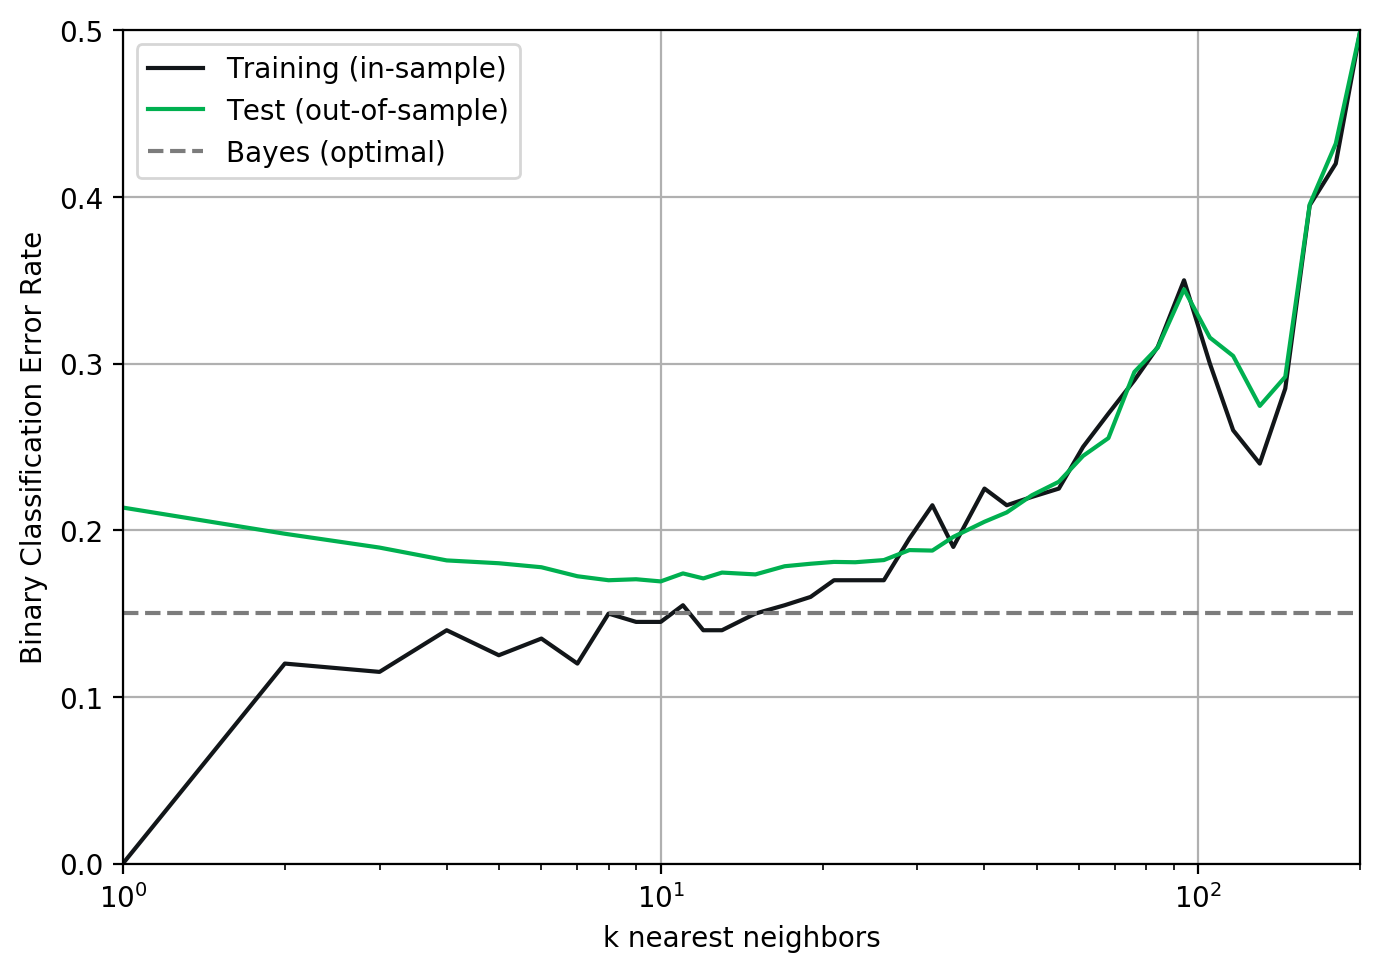
\includegraphics[width=3.80208in,height=3.83333in]{assignment4_files/figure-pdf/cell-4-output-1.png}

The hyperparameters we want to explore control the architecture of our
model and how our model is fit to our data. These hyperparameters
include the (a) learning rate, (b) batch size, and the (c)
regularization coefficient, as well as the (d) model architecture
hyperparameters (the number of layers and the number of nodes per
layer). We'll explore each of these and determine an optimized
configuration of the network for this problem through this exercise. For
all of the settings we'll explore and just, we'll assume the following
default hyperparameters for the model (we'll use scikit learn's
\href{https://scikit-learn.org/stable/modules/generated/sklearn.neural_network.MLPClassifier.html\#sklearn.neural_network.MLPClassifier.score}{\texttt{MLPClassifier}}
as our neural network model):

\begin{itemize}
\tightlist
\item
  \texttt{learning\_rate\_init} = 0.03
\item
  \texttt{hidden\_layer\_sizes} = (30,30) (two hidden layers, each with
  30 nodes)
\item
  \texttt{alpha} = 0 (regularization penalty)
\item
  \texttt{solver} = `sgd' (stochastic gradient descent optimizer)
\item
  \texttt{tol} = 1e-5 (this sets the convergence tolerance)
\item
  \texttt{early\_stopping} = False (this prevents early stopping)
\item
  \texttt{activation} = `relu' (rectified linear unit)
\item
  \texttt{n\_iter\_no\_change} = 1000 (this prevents early stopping)
\item
  \texttt{batch\_size} = 50 (size of the minibatch for stochastic
  gradient descent)
\item
  \texttt{max\_iter} = 500 (maximum number of epochs, which is how many
  times each data point will be used, not the number of gradient steps)
\end{itemize}

This default setting is our initial guess of what good values may be.
Notice there are many model hyperparameters in this list: any of these
could potentially be options to search over. We constrain the search to
those hyperparameters that are known to have a significant impact on
model performance.

\textbf{1.1. Visualize the impact of different hyperparameter choices on
classifier decision boundaries.} Visualize the impact of different
hyperparameter settings. Starting with the default settings above make
the following changes (only change one hyperparameter at a time). For
each hyperparameter value, plot the decision boundary on the training
data (you will need to train the model once for each parameter value):

\begin{enumerate}
\def\labelenumi{\arabic{enumi}.}
\tightlist
\item
  Vary the architecture (\texttt{hidden\_layer\_sizes}) by changing the
  number of nodes per layer while keeping the number of layers constant
  at 2: (2,2), (5,5), (30,30). Here (X,X) means a 2-layer network with X
  nodes in each layer.
\item
  Vary the learning rate: 0.0001, 0.01, 1
\item
  Vary the regularization: 0, 1, 10
\item
  Vary the batch size: 5, 50, 500
\end{enumerate}

This should produce 12 plots, altogether. For easier comparison, please
plot nodes \& layers combinations, learning rates, regularization
strengths, and batch sizes in four separate rows (with three columns
each representing a different value for each of those hyperparameters).

As you're exploring these settings, visit this website, the
\href{https://playground.tensorflow.org/\#activation=relu&batchSize=10&dataset=xor&regDataset=reg-plane&learningRate=0.03&regularizationRate=0&noise=20&networkShape=2,1&seed=0.89022&showTestData=false&discretize=false&percTrainData=50&x=true&y=true&xTimesY=false&xSquared=false&ySquared=false&cosX=false&sinX=false&cosY=false&sinY=false&collectStats=false&problem=classification&initZero=false&hideText=false&showTestData_hide=false}{Neural
Network Playground}, which will give you the chance to interactively
explore the impact of each of these parameters on a similar dataset to
the one we use in this exercise. The tool also allows you to adjust the
learning rate, batch size, regularization coefficient, and the
architecture and to see the resulting decision boundary and learning
curves. You can also visualize the model's hidden node output and its
weights, and it allows you to add in transformed features as well.
Experiment by adding or removing hidden layers and neurons per layer and
vary the hyperparameters.

\textbf{1.2. Manual (greedy) hyperparameter tuning I: manually optimize
hyperparameters that govern the learning process, one hyperparameter at
a time.} Now with some insight into which settings may work better than
others, let's more fully explore the performance of these different
settings in the context of our validation dataset through a manual
optimization process. Holding all else constant (with the default
settings mentioned above), vary each of the following parameters as
specified below. Train your algorithm on the training data, and evaluate
the performance of your trained algorithm on the validation dataset.
Here, overall accuracy is a reasonable performance metric since the
classes are balanced and we don't weight one type of error as more
important than the other; therefore, use the \texttt{score} method of
the \texttt{MLPClassifier} for this. Create plots of accuracy vs each
parameter you vary (this will result in three plots).

\begin{enumerate}
\def\labelenumi{\arabic{enumi}.}
\tightlist
\item
  Vary learning rate logarithmically from \(10^{-5}\) to \(10^{0}\) with
  20 steps
\item
  Vary the regularization parameter logarithmically from \(10^{-8}\) to
  \(10^2\) with 20 steps
\item
  Vary the batch size over the following values:
  \([1,3,5,10,20,50,100,250,500]\)
\end{enumerate}

For each of these cases:

\begin{itemize}
\tightlist
\item
  Based on the results, report your optimal choices for each of these
  hyperparameters and why you selected them.
\item
  Since neural networks can be sensitive to initialization values, you
  may notice these plots may be a bit noisy. Consider this when
  selecting the optimal values of the hyperparameters. If the noise
  seems significant, run the fit and score procedure multiple times
  (without fixing a random seed) and report the average. Rerunning the
  algorithm will change the initialization and therefore the output
  (assuming you do not set a random seed for that algorithm).
\item
  Use the chosen hyperparameter values as the new default settings for
  1.3 and 1.4.
\end{itemize}

\textbf{1.3. Manual (greedy) hyperparameter tuning II: manually optimize
hyperparameters that impact the model architecture.} Next, we want to
explore the impact of the model architecture on performance and optimize
its selection. This means varying two parameters at a time instead of
one as above. To do this, evaluate the validation accuracy resulting
from training the model using each pair of possible numbers of nodes per
layer and number of layers from the lists below. We will assume that for
any given configuration the number of nodes in each layer is the same
(e.g.~(2,2,2), which would be a 3-layer network with 2 hidden node in
each layer and (25,25) are valid, but (2,5,3) is not because the number
of hidden nodes varies in each layer). Use the manually optimized values
for learning rate, regularization, and batch size selected from 1.2.

\begin{itemize}
\item
  Number of nodes per layer: \([1,2,3,4,5,10,15,25,30]\)
\item
  Number of layers = \([1,2,3,4]\) Report the accuracy of your model on
  the validation data. For plotting these results, use heatmaps to plot
  the data in two dimensions. To make the heatmaps, you can use {[}this
  code for creating heatmaps{]}
  https://matplotlib.org/stable/gallery/images\_contours\_and\_fields/image\_annotated\_heatmap.html).
  Be sure to include the numerical values of accuracy in each grid
  square as shown in the linked example and label your x, y, and color
  axes as always. For these numerical values, round them to \textbf{2
  decimal places} (due to some randomness in the training process, any
  further precision is not typically meaningful).
\item
  When you select your optimized parameters, be sure to keep in mind
  that these values may be sensitive to the data and may offer the
  potential to have high variance for larger models. Therefore, select
  the model with the highest accuracy but lowest number of total model
  weights (all else equal, the simpler model is preferred).
\item
  What do the results show? Which parameters did you select and why?
\end{itemize}

\textbf{1.4. Manual (greedy) model selection and retraining.} Based the
optimal choice of hyperparameters, train your model with your optimized
hyperparameters on all the training data AND the validation data (this
is provided as \texttt{X\_train\_plus\_val} and
\texttt{y\_train\_plus\_val}).

\begin{itemize}
\tightlist
\item
  Apply the trained model to the test data and report the accuracy of
  your final model on the test data.
\item
  Plot an ROC curve of your performance (plot this with the curve in 1.5
  on the same set of axes you use for that question).
\end{itemize}

\textbf{1.5. Automated hyperparameter search through random search}. The
manual (greedy) approach (setting one or two parameters at a time
holding the rest constant), provides good insights into how the neural
network hyperparameters impacts model fitting for this particular
training process. However, it is limited in one very problematic way: it
depends heavily on a good ``default'' setting of the hyperparameters.
Those were provided for you in this exercise, but are not generally
know. Our manual optimization was somewhat greedy because we picked the
hyperparameters one at a time rather than looking at different
combinations of hyperparameters. Adopting such a pseudo-greedy approach
to that manual optimization also limits our ability to more deeply
search the hyperparameter space since we don't look at simultaneous
changes to multiple parameters. Now we'll use a popular hyperparameter
optimization tool to accomplish that: random search.

Random search is an excellent example of a hyperparameter optimization
search strategy that has
\href{https://www.jmlr.org/papers/volume13/bergstra12a/bergstra12a?ref=https://githubhelp.com}{been
shown to be more efficient} (requiring fewer training runs) than another
common approach: grid search. Grid search evaluates all possible
combinations of hyperparameters from lists of possible hyperparameter
settings - a very computationally expensive process. Yet another
attractive alternative is
\href{https://arxiv.org/abs/1807.02811}{Bayesian Optimization}, which is
an excellent hyperparameter optimization strategy but we will leave that
to the interested reader.

Our particular random search tool will be Scikit-Learn's
\href{https://scikit-learn.org/stable/modules/generated/sklearn.model_selection.RandomizedSearchCV.html\#sklearn.model_selection.RandomizedSearchCV}{\texttt{RandomizedSearchCV}}.
This performs random search employing cross validation for performance
evaluation (we will adjust this to ve a train/validation split).

Using \texttt{RandomizedSearchCV}, train on the training data while
validating on the validation data (see instructions below on how to
setup the train/validation split automatically). This tool will randomly
pick combinations of parameter values and test them out, returning the
best combination it finds as measured by performance on the validation
set. You can use
\href{https://scikit-learn.org/stable/auto_examples/model_selection/plot_randomized_search.html\#sphx-glr-auto-examples-model-selection-plot-randomized-search-py}{this
example} as a template for how to do this.

\begin{itemize}
\tightlist
\item
  To make this comparable to the training/validation setup used for the
  greedy optimization, we need to setup a training and validation split
  rather than use cross validation. To do this for
  \texttt{RandomSearchCV} we input the COMBINED training and validation
  dataset (\texttt{X\_train\_plus\_val}, and
  \texttt{y\_train\_plus\_val}) and we set the \texttt{cv} parameter to
  be the \texttt{train\_val\_split} variable we provided along with the
  dataset. This will setup the algorithm to make its assessments
  training just on the training data and evaluation on the validation
  data. Once \texttt{RandomSearchCV} completes its search, it will fit
  the model one more time to the combined training and validation data
  using the optimized parameters as we would want it to. \emph{Note: The
  object returned by running fit (the random search) is NOT the best
  estimator. You can access the best estimator through the attribute
  \texttt{.best\_estimator\_}, assuming that you did not pass
  \texttt{refit=False}.}
\item
  Set the number of iterations to at least 200 (you'll look at 200
  random pairings of possible hyperparameters). You can go as high as
  you want, but it will take longer the larger the value.
\item
  If you run this on Colab or any system with multiple cores, set the
  parameter \texttt{n\_jobs} to -1 to use all available cores for more
  efficient training through parallelization
\item
  You'll need to set the range or distribution of the parameters you
  want to sample from. Search over the same ranges as in previous
  problems. To tell the algorithm the ranges to search, use lists of
  values for candidate batch\_size, since those need to be integers
  rather than a range; the \texttt{loguniform} \texttt{scipy} function
  for setting the range of the learning rate and regularization
  parameter, and a list of tuples for the \texttt{hidden\_layer\_sizes}
  parameter, as you used in the greedy optimization.
\item
  Once the model is fit, use the \texttt{best\_params\_} property of the
  fit classifier attribute to extract the optimized values of the
  hyperparameters and report those and compare them to what was selected
  through the manual, greedy optimization.
\end{itemize}

For the final generalization performance assessment:

\begin{itemize}
\tightlist
\item
  State the accuracy of the optimized models on the test dataset
\item
  Plot the ROC curve corresponding to your best model on the test
  dataset through greedy hyperparameter section vs the model identified
  through random search (these curves should be on the same set of axes
  for comparison). In the legend of the plot, report the AUC for each
  curve. This should be one single graph with 3 curves (one for greedy
  search, one for random search, and one representing random chance).
  Please also provide AUC score for greedy research and random search.
\item
  Plot the final decision boundary for the greedy and random
  search-based classifiers along with the test dataset to demonstrate
  the shape of the final boundary
\item
  How did the generalization performance compare between the
  hyperparameters selected through the manual (greedy) search and the
  random search?
\end{itemize}

\subsection{Exercise 2 - Build and test your own Neural Network for
classification}\label{exercise-2---build-and-test-your-own-neural-network-for-classification}

\textbf{{[}30 points{]}}

There is no better way to understand how one of the core techniques of
modern machine learning works than to build a simple version of it
yourself. In this exercise you will construct and apply your own neural
network classifier. You may use numpy if you wish but no other
libraries.

\textbf{2.1} \emph{{[}10 points{]}} Create a neural network class that
follows the \texttt{scikit-learn} classifier convention by implementing
\texttt{fit}, \texttt{predict}, and \texttt{predict\_proba} methods.
Your \texttt{fit} method should run backpropagation on your training
data using stochastic gradient descent. Assume the activation function
is a sigmoid. Choose your model architecture to have two input nodes,
two hidden layers with five nodes each, and one output node.

To guide you in the right direction with this problem, please find a
skeleton of a neural network class below. You absolutely MAY use
additional methods beyond those suggested in this template, but the
methods listed below are the minimum required to implement the model
cleanly.

\textbf{Strategies for debugging}. One of the greatest challenges of
this implementations is that there are many parts and a bug could be
present in any of them. Here are some recommended tips:

\begin{itemize}
\tightlist
\item
  \emph{Development environment}. Consider using an Integrated
  Development Environment (IDE). I strongly recommend the use of VS Code
  and the Python debugging tools in that development environment.
\item
  \emph{Unit tests}. You are strongly encouraged to create unit tests
  for most modules. Without doing this will make your code extremely
  difficult to bug. You can create simple examples to feed through the
  network to validate it is correctly computing activations and node
  values. Also, if you manually set the weights of the model, you can
  even calculate backpropagation by hand for some simple examples
  (admittedly, that unit test would be challenging and is optional, but
  a unit test is possible).
\item
  \emph{Compare against a similar architecture}. You can also verify the
  performance of your overall neural network by comparing it against the
  \texttt{scikit-learn} implementation and using the same architecture
  and parameters as your model (your model outputs will certainly not be
  identical, but they should be somewhat similar for similar parameter
  settings).
\end{itemize}

\begin{tcolorbox}[enhanced jigsaw, titlerule=0mm, opacityback=0, colbacktitle=quarto-callout-important-color!10!white, coltitle=black, rightrule=.15mm, leftrule=.75mm, bottomrule=.15mm, colframe=quarto-callout-important-color-frame, toptitle=1mm, left=2mm, bottomtitle=1mm, opacitybacktitle=0.6, title=\textcolor{quarto-callout-important-color}{\faExclamation}\hspace{0.5em}{Important Note}, toprule=.15mm, arc=.35mm, colback=white, breakable]

Building a neural net is a valuable learning opportunity, but a time
intensive process. Due to the depth of effort this question requires,
some students may choose not to complete this section. It's only worth
10 points, which is not proportional to the time it takes to get it
working, and that's by design. If you choose not to build your own
neural network, or if your neural network is not functional prior to
submission, then use the \texttt{scikit-learn} implementation instead in
the questions below; where it asks to compare to \texttt{scikit-learn},
compare against a random forest classifier instead.

Simply write ``OMITTED'' in your response to this question to indicate
that you did not write your own neural network.

\end{tcolorbox}

\begin{Shaded}
\begin{Highlighting}[]
\CommentTok{\# neural network class skeleton code}

\KeywordTok{class}\NormalTok{ myNeuralNetwork(}\BuiltInTok{object}\NormalTok{):}
    
    \KeywordTok{def} \FunctionTok{\_\_init\_\_}\NormalTok{(}\VariableTok{self}\NormalTok{, n\_in, n\_layer1, n\_layer2, n\_out, learning\_rate}\OperatorTok{=}\NormalTok{):}
        \CommentTok{\textquotesingle{}\textquotesingle{}\textquotesingle{}\_\_init\_\_}
\CommentTok{        Class constructor: Initialize the parameters of the network including}
\CommentTok{        the learning rate, layer sizes, and each of the parameters}
\CommentTok{        of the model (weights, placeholders for activations, inputs, }
\CommentTok{        deltas for gradients, and weight gradients). This method}
\CommentTok{        should also initialize the weights of your model randomly}
\CommentTok{            Input:}
\CommentTok{                n\_in:          number of inputs}
\CommentTok{                n\_layer1:      number of nodes in layer 1}
\CommentTok{                n\_layer2:      number of nodes in layer 2}
\CommentTok{                n\_out:         number of output nodes}
\CommentTok{                learning\_rate: learning rate for gradient descent}
\CommentTok{            Output:}
\CommentTok{                none}
\CommentTok{        \textquotesingle{}\textquotesingle{}\textquotesingle{}}
            
    \KeywordTok{def}\NormalTok{ forward\_propagation(}\VariableTok{self}\NormalTok{, x):}
        \CommentTok{\textquotesingle{}\textquotesingle{}\textquotesingle{}forward\_propagation}
\CommentTok{        Takes a vector of your input data (one sample) and feeds}
\CommentTok{        it forward through the neural network, calculating activations and}
\CommentTok{        layer node values along the way.}
\CommentTok{            Input:}
\CommentTok{                x: a vector of data representing 1 sample [n\_in x 1]}
\CommentTok{            Output:}
\CommentTok{                y\_hat: a vector (or scaler of predictions) [n\_out x 1]}
\CommentTok{                (typically n\_out will be 1 for binary classification)}
\CommentTok{        \textquotesingle{}\textquotesingle{}\textquotesingle{}}
    
    \KeywordTok{def}\NormalTok{ compute\_loss(}\VariableTok{self}\NormalTok{, X, y):}
        \CommentTok{\textquotesingle{}\textquotesingle{}\textquotesingle{}compute\_loss}
\CommentTok{        Computes the current loss/cost function of the neural network}
\CommentTok{        based on the weights and the data input into this function.}
\CommentTok{        To do so, it runs the X data through the network to generate}
\CommentTok{        predictions, then compares it to the target variable y using}
\CommentTok{        the cost/loss function}
\CommentTok{            Input:}
\CommentTok{                X: A matrix of N samples of data [N x n\_in]}
\CommentTok{                y: Target variable [N x 1]}
\CommentTok{            Output:}
\CommentTok{                loss: a scalar measure of loss/cost}
\CommentTok{        \textquotesingle{}\textquotesingle{}\textquotesingle{}}
    
    \KeywordTok{def}\NormalTok{ backpropagate(}\VariableTok{self}\NormalTok{, x, y):}
        \CommentTok{\textquotesingle{}\textquotesingle{}\textquotesingle{}backpropagate}
\CommentTok{        Backpropagate the error from one sample determining the gradients}
\CommentTok{        with respect to each of the weights in the network. The steps for}
\CommentTok{        this algorithm are:}
\CommentTok{            1. Run a forward pass of the model to get the activations }
\CommentTok{               Corresponding to x and get the loss functionof the model }
\CommentTok{               predictions compared to the target variable y}
\CommentTok{            2. Compute the deltas (see lecture notes) and values of the}
\CommentTok{               gradient with respect to each weight in each layer moving}
\CommentTok{               backwards through the network}
\CommentTok{    }
\CommentTok{            Input:}
\CommentTok{                x: A vector of 1 samples of data [n\_in x 1]}
\CommentTok{                y: Target variable [scalar]}
\CommentTok{            Output:}
\CommentTok{                loss: a scalar measure of th loss/cost associated with x,y}
\CommentTok{                      and the current model weights}
\CommentTok{        \textquotesingle{}\textquotesingle{}\textquotesingle{}}
        
    \KeywordTok{def}\NormalTok{ stochastic\_gradient\_descent\_step(}\VariableTok{self}\NormalTok{):}
        \CommentTok{\textquotesingle{}\textquotesingle{}\textquotesingle{}stochastic\_gradient\_descent\_step [OPTIONAL {-} you may also do this}
\CommentTok{        directly in backpropagate]}
\CommentTok{        Using the gradient values computed by backpropagate, update each}
\CommentTok{        weight value of the model according to the familiar stochastic}
\CommentTok{        gradient descent update equation.}
\CommentTok{        }
\CommentTok{        Input: none}
\CommentTok{        Output: none}
\CommentTok{        \textquotesingle{}\textquotesingle{}\textquotesingle{}}
    
    \KeywordTok{def}\NormalTok{ fit(}\VariableTok{self}\NormalTok{, X, y, max\_epochs}\OperatorTok{=}\NormalTok{, learning\_rate}\OperatorTok{=}\NormalTok{, get\_validation\_loss}\OperatorTok{=}\NormalTok{):}
        \CommentTok{\textquotesingle{}\textquotesingle{}\textquotesingle{}fit}
\CommentTok{            Input:}
\CommentTok{                X: A matrix of N samples of data [N x n\_in]}
\CommentTok{                y: Target variable [N x 1]}
\CommentTok{            Output:}
\CommentTok{                training\_loss:   Vector of training loss values for each epoch}
\CommentTok{                validation\_loss: Vector of validation loss values for each epoch}
\CommentTok{                                 [optional output if get\_validation\_loss==True]}
\CommentTok{        \textquotesingle{}\textquotesingle{}\textquotesingle{}}
            
    \KeywordTok{def}\NormalTok{ predict\_proba(}\VariableTok{self}\NormalTok{, X):}
        \CommentTok{\textquotesingle{}\textquotesingle{}\textquotesingle{}predict\_proba}
\CommentTok{        Compute the output of the neural network for each sample in X, with the }
\CommentTok{        last layer\textquotesingle{}s sigmoid activation providing an estimate of the target }
\CommentTok{        output between 0 and 1}
\CommentTok{            Input:}
\CommentTok{                X: A matrix of N samples of data [N x n\_in]}
\CommentTok{            Output:}
\CommentTok{                y\_hat: A vector of class predictions between 0 and 1 [N x 1]}
\CommentTok{        \textquotesingle{}\textquotesingle{}\textquotesingle{}}
    
    \KeywordTok{def}\NormalTok{ predict(}\VariableTok{self}\NormalTok{, X, decision\_thresh}\OperatorTok{=}\NormalTok{):}
        \CommentTok{\textquotesingle{}\textquotesingle{}\textquotesingle{}predict}
\CommentTok{        Compute the output of the neural network prediction for }
\CommentTok{        each sample in X, with the last layer\textquotesingle{}s sigmoid activation }
\CommentTok{        providing an estimate of the target output between 0 and 1, }
\CommentTok{        then thresholding that prediction based on decision\_thresh}
\CommentTok{        to produce a binary class prediction}
\CommentTok{            Input:}
\CommentTok{                X: A matrix of N samples of data [N x n\_in]}
\CommentTok{                decision\_threshold: threshold for the class confidence score}
\CommentTok{                                    of predict\_proba for binarizing the output}
\CommentTok{            Output:}
\CommentTok{                y\_hat: A vector of class predictions of either 0 or 1 [N x 1]}
\CommentTok{        \textquotesingle{}\textquotesingle{}\textquotesingle{}}
    
    \KeywordTok{def}\NormalTok{ sigmoid(}\VariableTok{self}\NormalTok{, X):}
        \CommentTok{\textquotesingle{}\textquotesingle{}\textquotesingle{}sigmoid}
\CommentTok{        Compute the sigmoid function for each value in matrix X}
\CommentTok{            Input:}
\CommentTok{                X: A matrix of any size [m x n]}
\CommentTok{            Output:}
\CommentTok{                X\_sigmoid: A matrix [m x n] where each entry corresponds to the}
\CommentTok{                           entry of X after applying the sigmoid function}
\CommentTok{        \textquotesingle{}\textquotesingle{}\textquotesingle{}}
    
    \KeywordTok{def}\NormalTok{ sigmoid\_derivative(}\VariableTok{self}\NormalTok{, X):}
        \CommentTok{\textquotesingle{}\textquotesingle{}\textquotesingle{}sigmoid\_derivative}
\CommentTok{        Compute the sigmoid derivative function for each value in matrix X}
\CommentTok{            Input:}
\CommentTok{                X: A matrix of any size [m x n]}
\CommentTok{            Output:}
\CommentTok{                X\_sigmoid: A matrix [m x n] where each entry corresponds to the}
\CommentTok{                           entry of X after applying the sigmoid derivative }
\CommentTok{                           function}
\CommentTok{        \textquotesingle{}\textquotesingle{}\textquotesingle{}}
\end{Highlighting}
\end{Shaded}

\textbf{2.2}. Apply your neural network.

\begin{itemize}
\tightlist
\item
  Create training, validation, and test datasets using
  \texttt{sklearn.datasets.make\_moons(N,\ noise=0.20)} data, where
  \(N_{train} = 500\) and \(N_{test} = 100\). The validation dataset
  should be a portion of your training dataset that you hold out for
  hyperparameter tuning.
\item
  \textbf{Cost function plots}. Train and validate your model on this
  dataset plotting your training and validation cost learning curves on
  the same set of axes. This is the training and validation error for
  each epoch of stochastic gradient descent, where an epoch represents
  having trained on each of the training samples one time.
\item
  Tune the learning rate and number of training epochs for your model to
  improve performance as needed. You're free to use any methods you deem
  fit to tune your hyperparameters like grid search, random search,
  Bayesian optimization etc.
\item
  \textbf{Decision boundary plots}. In two subplots, plot the training
  data on one subplot and the validation data on the other subplot. On
  each plot, also plot the decision boundary from your neural network
  trained on the training data.
\item
  \textbf{ROC Curve plots}. Report your performance on the test data
  with an ROC curve and the corresponding AUC score. Compare against the
  \texttt{scikit-learn} \texttt{MLPClassifier} trained with the same
  parameters on the same set of axes and include the chance diagonal.
  \emph{Note: if you chose not to build your own neural network in part
  (a) above, or if your neural network is not functional prior to
  submission, then use the \texttt{scikit-learn} \texttt{MLPClassifier}
  class instead for the neural network and compare it against a random
  forest classifier instead. Be sure to set the hidden layer sizes,
  epochs, and learning rate for that model, if so.}
\item
  \textbf{Remember to retrain your model.} After selecting your
  hyperparameters using the validation data set, when evaluating the
  final performance on the ROC curve, it's good practice to retrain your
  model with the selected hyperparameters on the train + validation
  dataset, before evaluating on the test data.
\end{itemize}

Note if you opted not to build your own neural network: in this case,
for hyperparameter tuning, we recommend using the \texttt{partial\_fit}
method to train your model for every epoch. Partial fit allows you to
incrementally fit on one sample at a time.

\textbf{2.3}. Suggest two ways in which you neural network
implementation could be improved: are there any options we discussed in
class that were not included in your implementation that could improve
performance?




\end{document}
